% Copyright 2004 by Till Tantau <tantau@users.sourceforge.net>.
%
% In principle, this file can be redistributed and/or modified under
% the terms of the GNU Public License, version 2.
%
% However, this file is supposed to be a template to be modified
% for your own needs. For this reason, if you use this file as a
% template and not specifically distribute it as part of a another
% package/program, I grant the extra permission to freely copy and
% modify this file as you see fit and even to delete this copyright
% notice. 

\documentclass{beamer}

\usepackage{graphicx}

% There are many different themes available for Beamer. A comprehensive
% list with examples is given here:
% http://deic.uab.es/~iblanes/beamer_gallery/index_by_theme.html
% You can uncomment the themes below if you would like to use a different
% one:
%\usetheme{AnnArbor}
%\usetheme{Antibes}
%\usetheme{Bergen}
%\usetheme{Berkeley}
%\usetheme{Berlin}
%\usetheme{Boadilla}
%\usetheme{boxes}
%\usetheme{CambridgeUS}
%\usetheme{Copenhagen}
%\usetheme{Darmstadt}
%\usetheme{default}
%\usetheme{Frankfurt}
%\usetheme{Goettingen}
%\usetheme{Hannover}
%\usetheme{Ilmenau}
%\usetheme{JuanLesPins}
%\usetheme{Luebeck}
%\usetheme{Madrid}
%\usetheme{Malmoe}
%\usetheme{Marburg}
%\usetheme{Montpellier}
%\usetheme{PaloAlto}
%\usetheme{Pittsburgh}
%\usetheme{Rochester}
\usetheme{Singapore}
%\usetheme{Szeged}
%\usetheme{Warsaw}

\addtobeamertemplate{navigation symbols}{}{%
    \usebeamerfont{footline}%
    \usebeamercolor[fg]{footline}%
    \hspace{1em}%
    \insertframenumber/\inserttotalframenumber
}

\title{Towards Nonmonotonic Relational Learning from Knowledge Graphs}

% A subtitle is optional and this may be deleted
\subtitle{}

\author{Hai Dang Tran\inst{1}}
% - Give the names in the same order as the appear in the paper.
% - Use the \inst{?} command only if the authors have different
%   affiliation.

\institute[Max Planck Institute for Informatics] % (optional, but mostly needed)
{
  \inst{1}%
  Saarland University\\
  Max Planck Institute for Informatics
}
% - Use the \inst command only if there are several affiliations.
% - Keep it simple, no one is interested in your street address.

\date{2016}
% - Either use conference name or its abbreviation.
% - Not really informative to the audience, more for people (including
%   yourself) who are reading the slides online

\subject{Information System}
% This is only inserted into the PDF information catalog. Can be left
% out. 

% If you have a file called "university-logo-filename.xxx", where xxx
% is a graphic format that can be processed by latex or pdflatex,
% resp., then you can add a logo as follows:

% \pgfdeclareimage[height=1cm]{university-logo}{mpi-logo.png}
% \logo{\pgfuseimage{university-logo}}

% Delete this, if you do not want the table of contents to pop up at
% the beginning of each subsection:
\AtBeginSubsection[]
{
  \begin{frame}<beamer>{Outline}
    \tableofcontents[currentsection,currentsubsection]
  \end{frame}
}

% Let's get started
\begin{document}

\begin{frame}
  \titlepage
\end{frame}

\begin{frame}{Outline}
  \tableofcontents
  % You might wish to add the option [pausesections]
\end{frame}

% Section and subsections will appear in the presentation overview
% and table of contents.
\section{System Overview}

\begin{frame}{System Overview}

\begin{figure}[h]
	\centering
	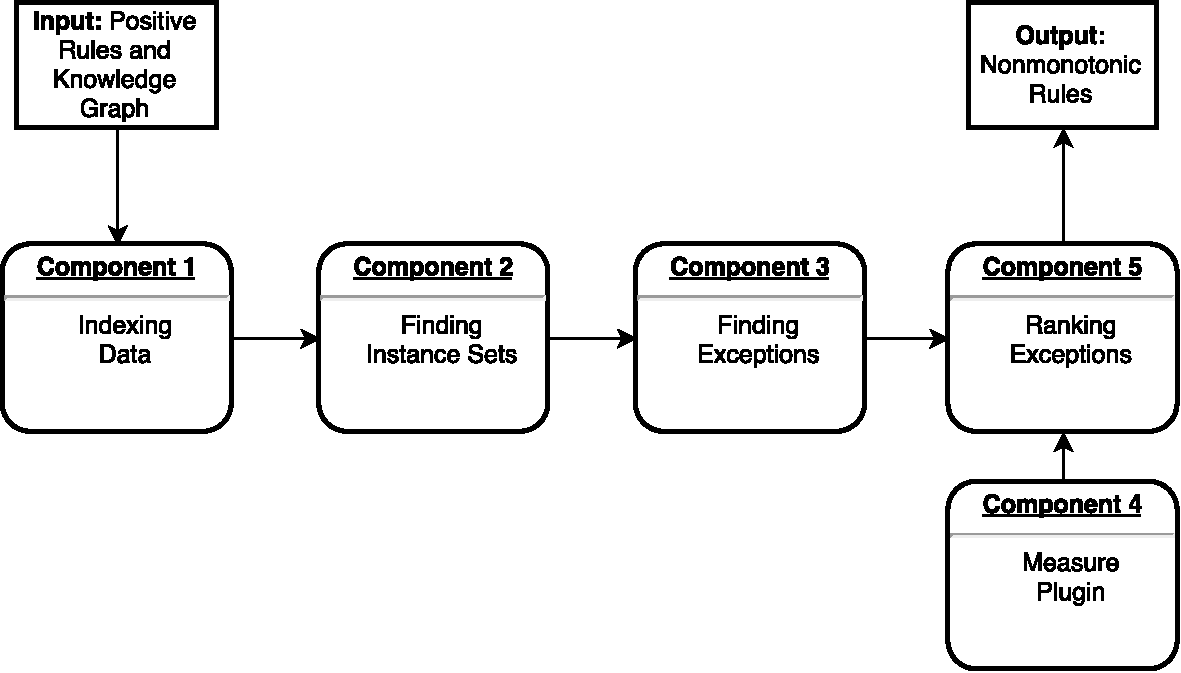
\includegraphics[page=1,width=.75\textwidth]{overview.pdf}
	\caption{Components in the System}
\end{figure}

\end{frame}

\section{System Description}

\subsection{Indexing Data}

\begin{frame}{Indexing Data}

Goal: support searching over a dataset.

Intuition:
\begin{itemize}
	\item Inverted indexing from term to document in IR systems.
  	\item In this problem, a triple is a document.
  	\item Find corresponding predicates given subject, object.
\end{itemize}

\end{frame}

\subsection{Finding Instance Sets}

\begin{frame}{Finding Instance Sets}

\begin{figure}[h]
	\centering
	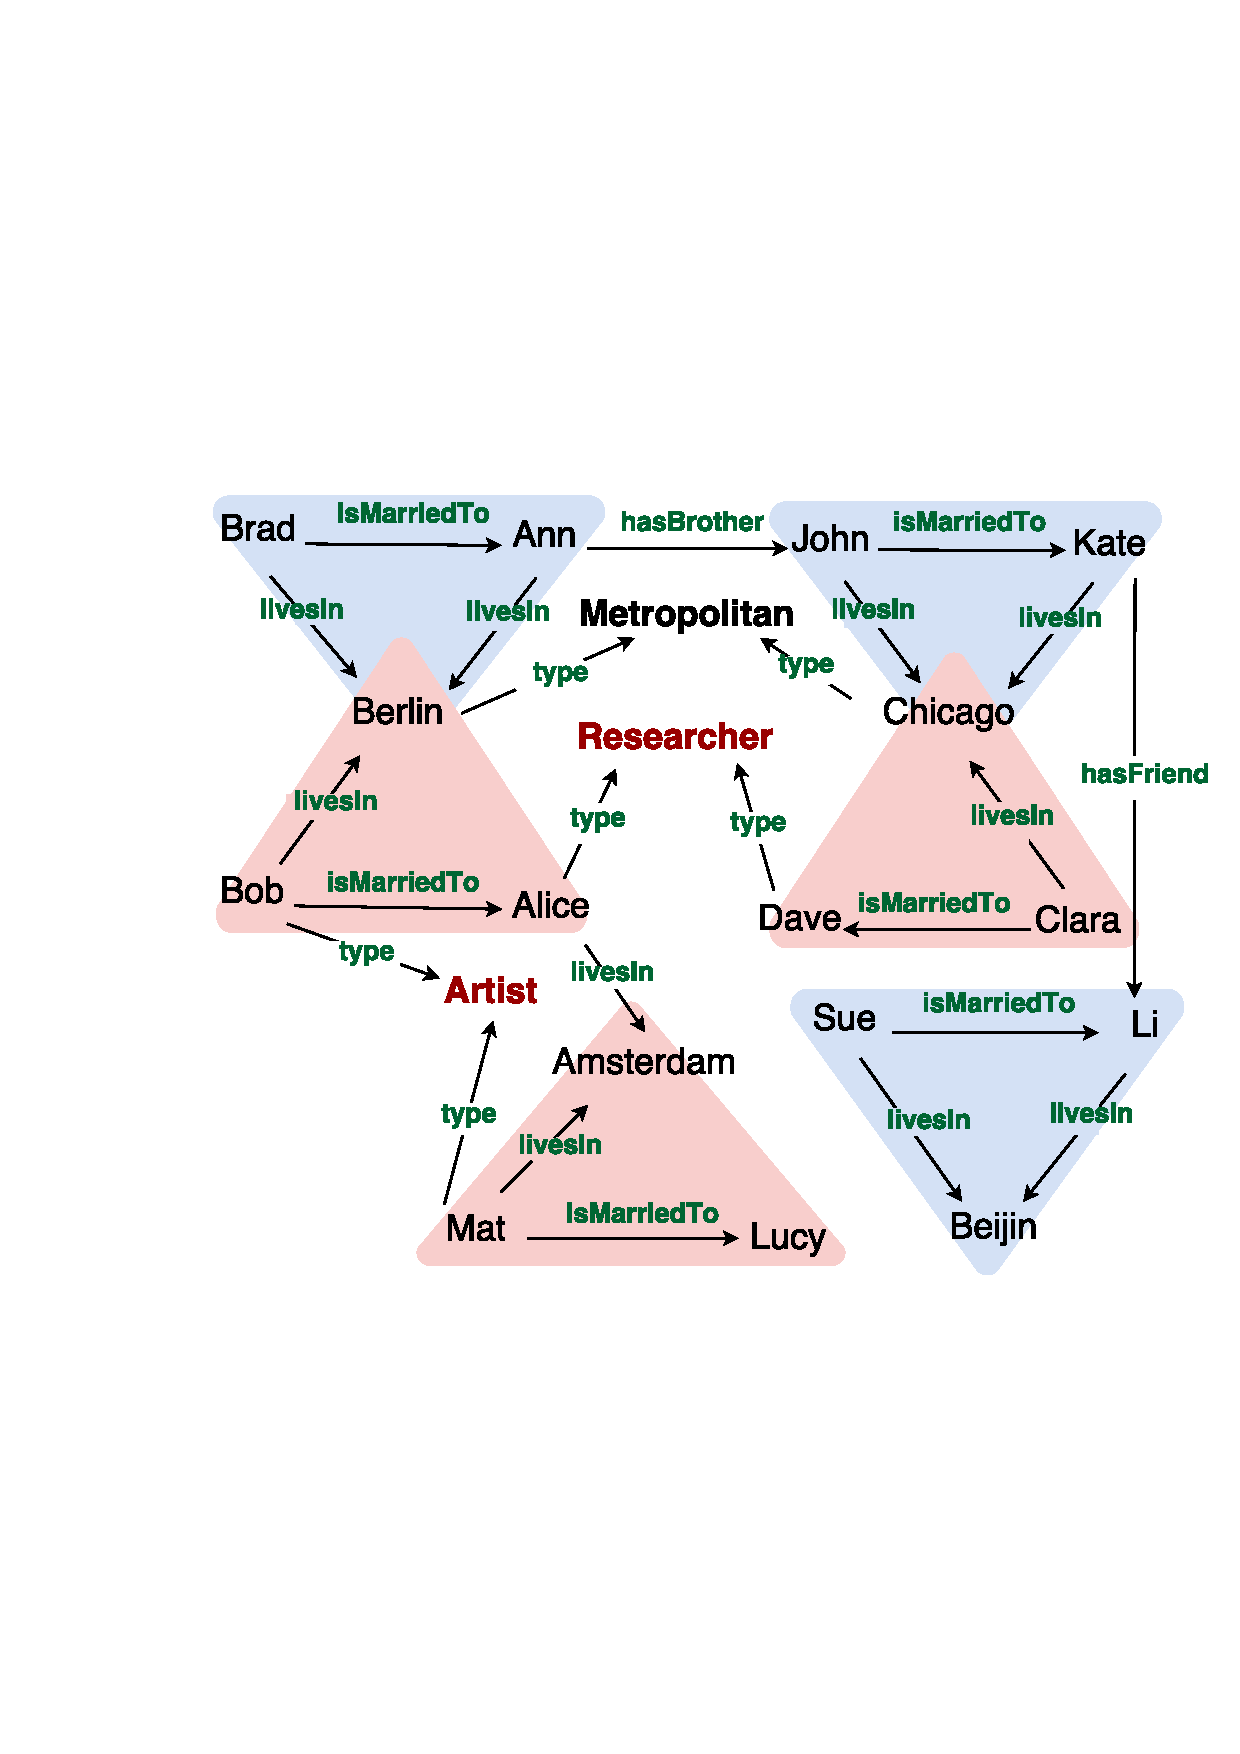
\includegraphics[page=1,width=.5\textwidth]{example.pdf}
	\caption{A KG Example with rule \textit{livesIn(X, Z) $\leftarrow$ isMarriedTo(Y, X), livesIn(Y, Z)}, Source: ILP Paper.}
\end{figure}

\end{frame}

\begin{frame}{Finding Instance Sets}

Horn rule $r$: \textit{H(X, Z) $\leftarrow$ P(X, Y) $\wedge$ Q(Y, Z)}.
\begin{itemize}
	\item Traverse all substitutions for $Y$.
	\item Find list of $Y$ from $PX$ based on indexing.
	\item Find list of $Z$ from $QY$ based on indexing.
	\item Check \textit{$\langle$X H Z$\rangle$} in the graph or not.
	\item Classify \textit{$\langle$X Z$\rangle$} into $NS(r)$ and $ABS(r)$.
\end{itemize}

\end{frame}

\subsection{Finding Exceptions}

\begin{frame}{Finding Exceptions}

Three exception types:
\begin{itemize}
	\item \textit{EWS(r, G, X), EWS(r, G, Y)} as unary predicates for $X$, $Z$.
	\item {
		\textit{EWS(r, G, $\langle$X Z$\rangle$)} as binary predicate for \textit{$\langle$X Z$\rangle$}.
		\pause
	}
\end{itemize}

How to find \textit{EWS(r, G, $\langle$X Z$\rangle$)}?
\begin{itemize}
	\item Let $E^+ = \{P | \exists (X, Z) \in ABS(r): P(X, Z) \in G\}$.
	\item Let $E^- = \{P | \exists (X, Z) \in NS(r): P(X, Z) \in G\}$.
	\item Then \textit{EWS(r, G, $\langle$X Z$\rangle$)} $= E^+ \setminus E^-$.
\end{itemize}

To find $E^+$, we use data indexing again.

\end{frame}

\begin{frame}{Finding Exceptions}

\begin{figure}[h]
	\centering
	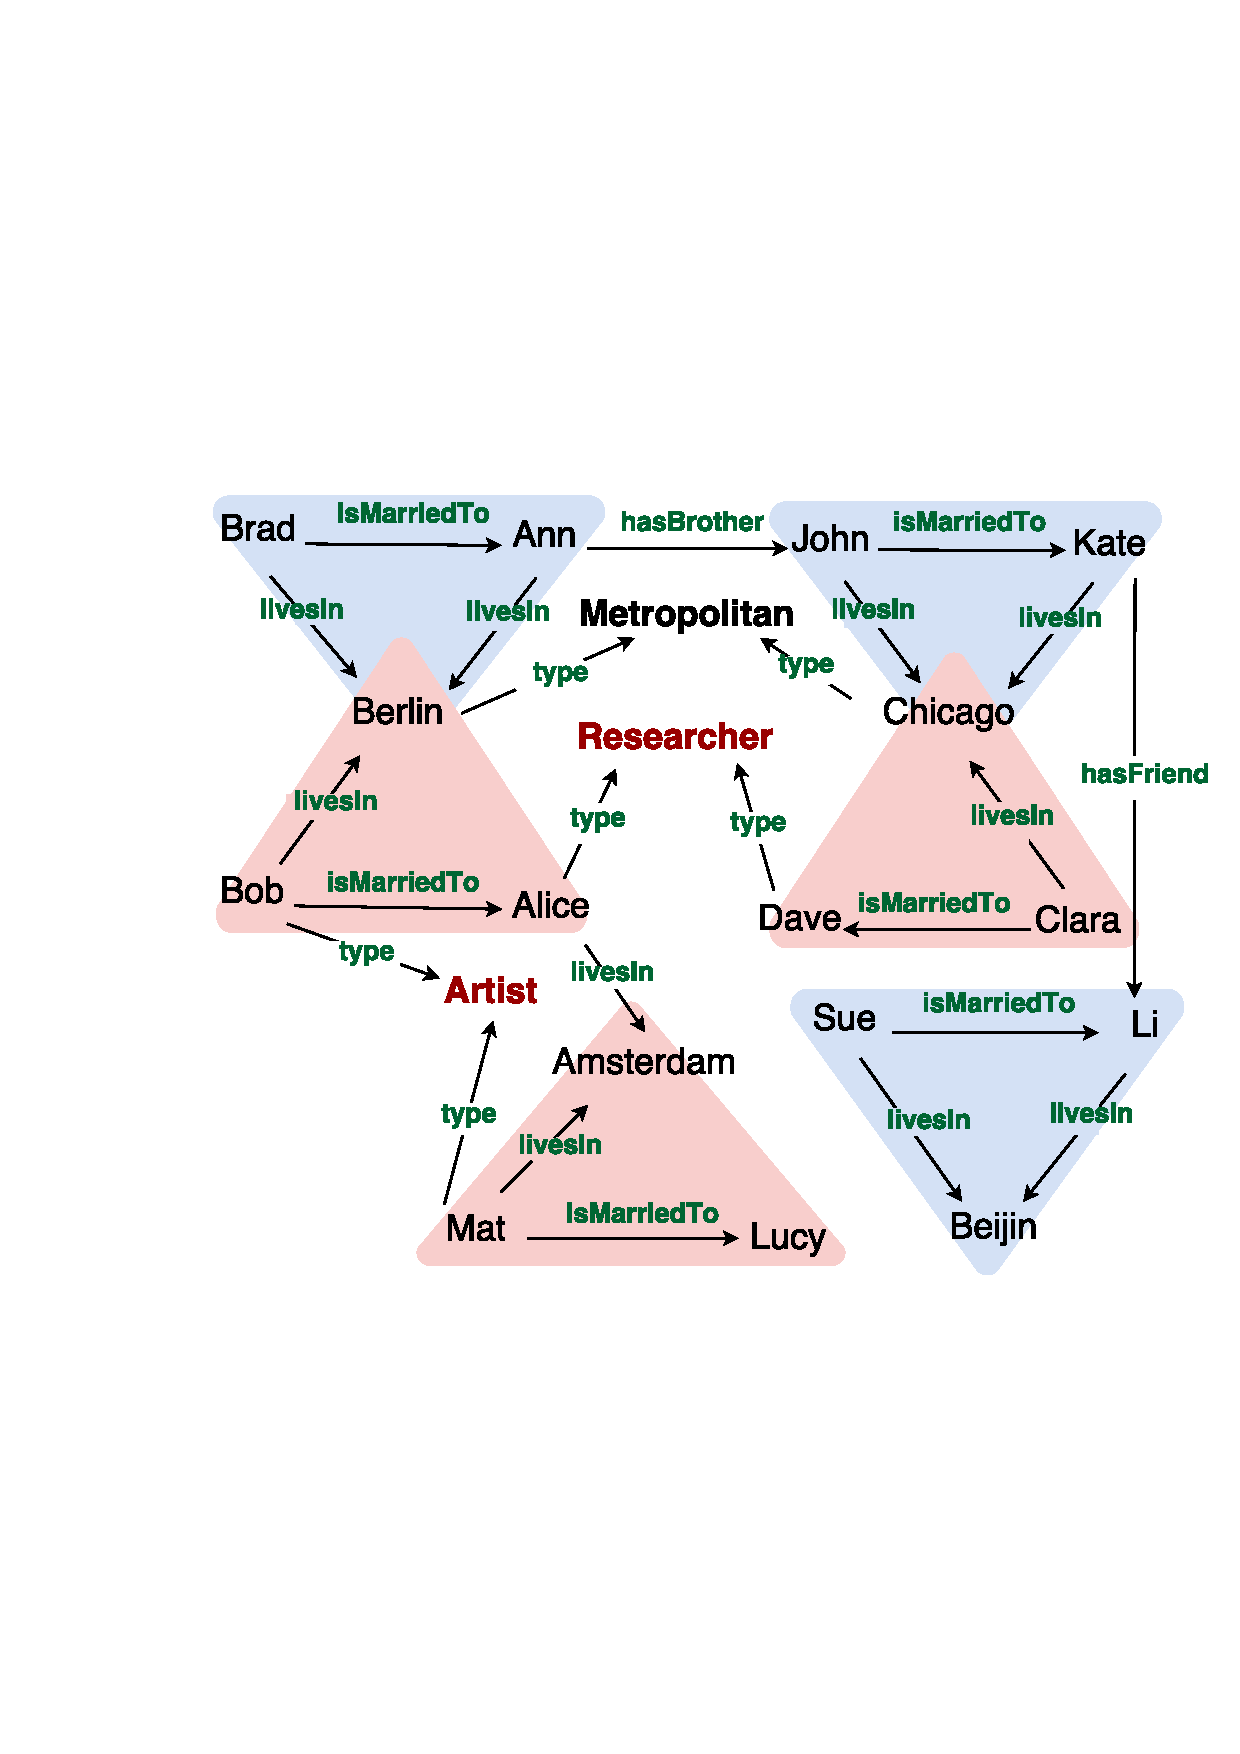
\includegraphics[page=1,width=.5\textwidth]{example.pdf}
	\caption{A KG Example, Source: ILP Paper.}
\end{figure}

\textit{livesIn(X, Z) $\leftarrow$ isMarriedTo(Y, X), livesIn(Y, Z)}, exception candidates: \textit{Researcher, Artist}.

\end{frame}

\subsection{Measure Plugin}

\begin{frame}{Measure Plugin}

Goal: test different measures.

Reasons:
\begin{itemize}
	\item Confidence measure is not good for prediction~\cite{ref1}.
	\item Current measure is conviction, $conv(r) = \frac{1 - supp(r)}{1 - conf(r)}$.
	\item {
		Other measures can be plugged in the system~\cite{ref2}.
		\pause
	}
\end{itemize}

Score function for ranking:
\begin{itemize}
	\item $score(r) = \frac{conv(r) + conv(r^{aux})}{2}$.
	\item Sort exceptions in decreasing order of score function.
	\item If there is a tie, sort by decreasing order of $conv(r)$.
\end{itemize}

\end{frame}

\subsection{Ranking Exceptions}

\begin{frame}{Ranking Exceptions}

Ordered Partial Materialization (OPM):
\begin{itemize}
	\item Sort all positive rules according to decreasing order of conviction.
	\item For each rule $r$, we use original facts and predicted ones (updated KG) from previous rules to infer $NS(r), ABS(r)$.
	\item Rank exceptions based on the score function over updated KG.
	\item Choose all exceptions of $r$ to infer new facts.
\end{itemize}

\end{frame}

\section{Current Result and Future Work}

\begin{frame}{Current Result and Future Work}

Some mined rules:
\begin{itemize}
	\item {
		\textit{writtenBy(X , Z) $\leftarrow$ hasPredecessor(X , Y), writtenBy(Y , Z), not isAmericanFilm(X)}.
	}
	\item {
		\textit{actedIn(X , Z) $\leftarrow$ isMarriedTo(X , Y), directed(Y, Z), not isSilentFilmActor(X)}.
		\pause
	}
\end{itemize}

Several works need to be done:
\begin{itemize}
	\item Experiments with other datasets, e.g, YAGO and Freebase.
	\item Enable more forms for given positive rules.
	\item Test with other predictive measures.
\end{itemize}

\end{frame}

\section*{References}

\begin{frame}{Reference}
  \frametitle<presentation>{For Further Reading}
  \begin{thebibliography}{10}

  \beamertemplatearticlebibitems
  % Followed by interesting articles. Keep the list short. 

  \bibitem{ref1}
    Azevedo et al.
    \newblock Comparing Rule Measures for Predictive Association Rules.
    \newblock {\em Proceedings of ECML}, 510--517,
    2007.

  \bibitem{ref2}
    Todorovski et al.
    \newblock Predictive Performance of Weighted Relative Accuracy.
    \newblock {\em 4th European Conference, PKDD}, 255--264,
    2000.

  \end{thebibliography}
\end{frame}

\end{document}